%!TeX root =  ../../thesis.tex

\section{Jednodeskové počítače v kontextu IoT}
Internet věcí (IoT) označuje síť vzájemně propojených fyzických zařízení, která jsou schopna sbírat a sdílet data pomocí vestavěných senzorů a komunikačních technologií. Tyto zařízení mohou být od všedních předmětů až po složité průmyslové systémy.
Základem těchto zařízení bývají jednodeskové počítače nebo po případě mikrokontroléry.\\
Jednodeskové počítače jsou zařízení obsahující veškeré potřebné komponenty pro provoz a řízení výpočetních procesů na jediné desce plošného spoje a mezi známé příklady patří Arduino, Raspberry Pi nebo ESP32.

%!TeX root =  ../../thesis.tex

\subsection{Raspberry Pi}
Raspberry Pi je značka jednodeskových počítačů na kterých je primárně operační systém Raspberry Pi OS (dříve Raspbian). Jedná se odlehčenou linuxovou distribuci, která je založena na linuxové distribuci Debian, které je známá svou stabilitou. Raspberry Pi je původem ze Spojeného Království a je vhodné pro začátečníky v IoT, jelikož použití je intuitivnější a také se na něm dá vyvíjet pomocí Pythonu.
\begin{figure}[H]
	\centering
	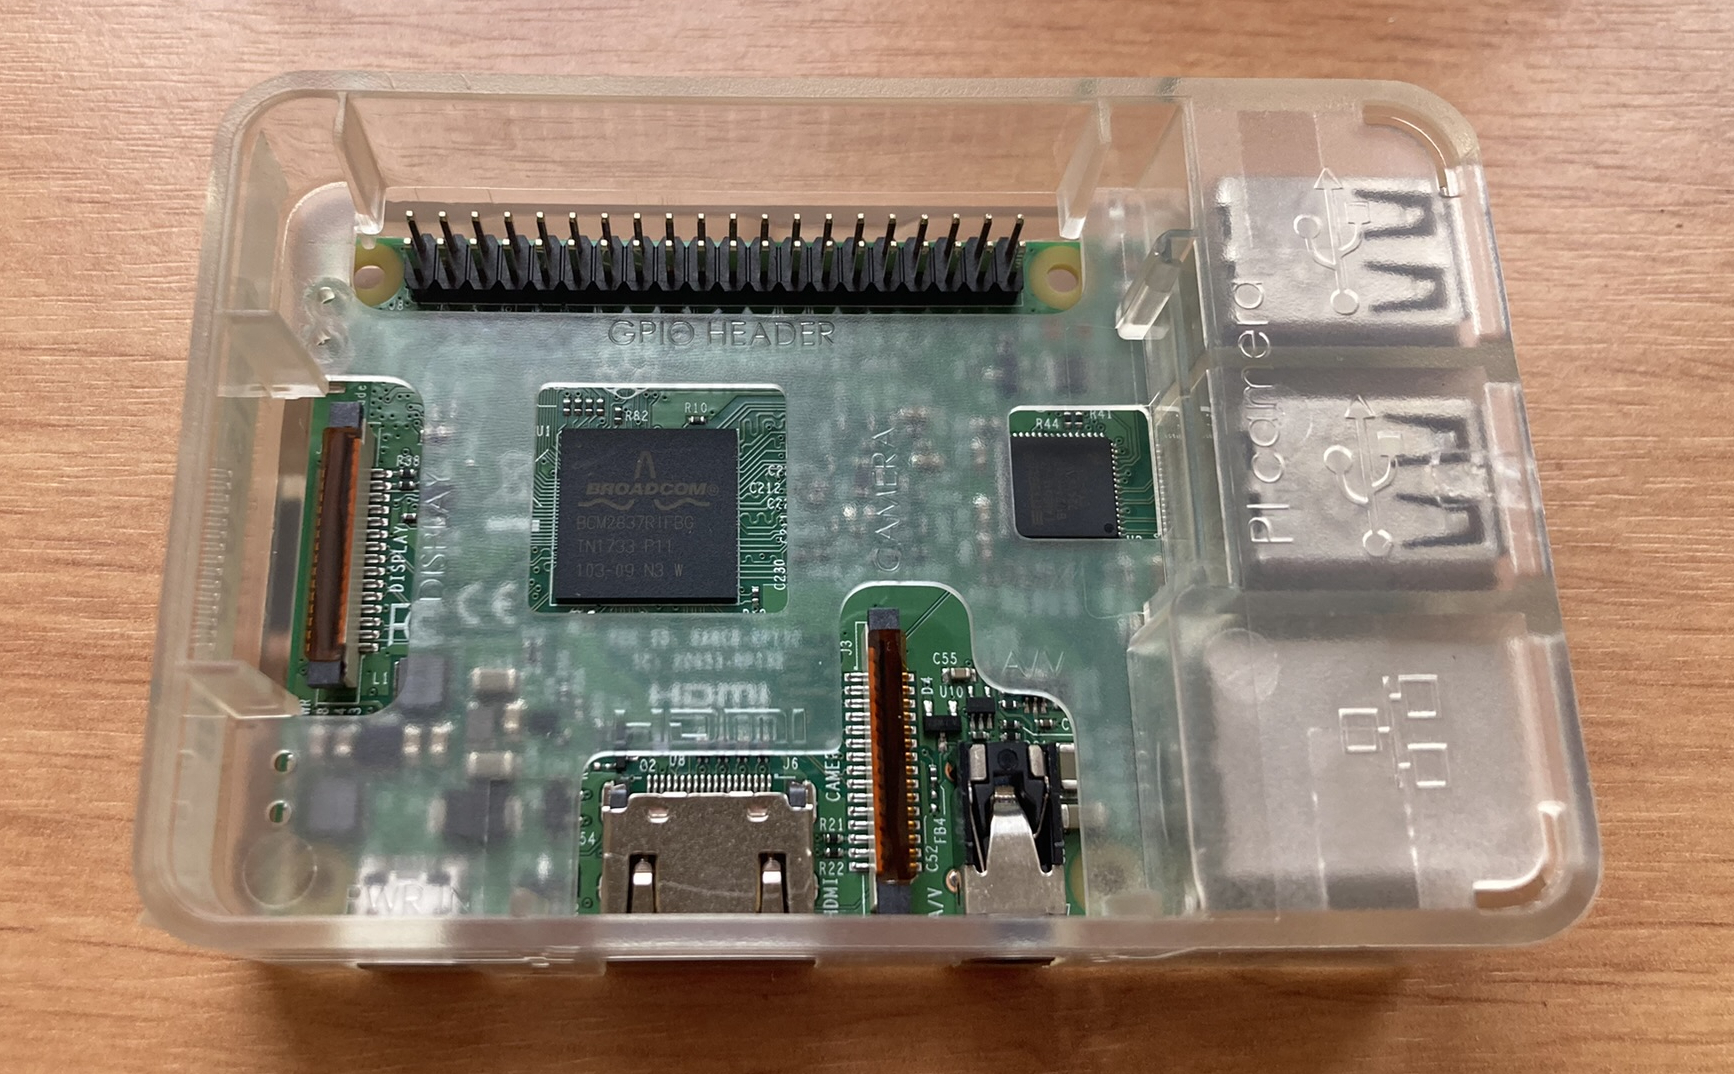
\includegraphics[width=0.9\textwidth]{pictures/rasp.jpeg}
    	\caption{Raspberry Pi}
   	\label{fig:rasPI}
\end{figure}
Na obrázku \ref{fig:rasPI} vidíme Rapsberry PI, které je v plastovém obalu s výřezy pro přístup na IO, včetně pinového headeru, na který se dá připojit shield s polem led žároviček. Také vidíme USB a RJ-45 konektor a další konektory, ovšem já se momentálně nevěnuji práci s Rapsberry Pi, tudíž mu v této bakalářské práci nebudu věnovat tolik pozornosti, nicméně jej bylo důležité zmínit, jelikož patří mezi významné jednodeskové počítače.
%!TeX root =  ../../thesis.tex

\section{Arduino}
Základem testeru je mikrokontrolér od značky Arduino model \ardMeg. Tento model disponuje velkým počtem pinům, na které je možné připojit různá zařízení a následně je ovládat mikrokontrolérem. Mikrokontroléry Arduino se programují pomocí C/C++. Já firmware pro toto tester píši v C++.

\begin{figure}[h!]
	\centering
	
\includegraphics[width=\textwidth]{pictures/placeHolderFHD.png}
    	\caption{\ardMeg}
   	\label{fig:arduinoMega}
\end{figure}


%\subsection*{Ino file}
%\lstinputlisting[language=C++, caption={Code.ino}, label={lst:code}]{../code/Code.ino}

%\subsubsection*{Co je to Ino file?}
%Ino file je soubor skatche pro Arduino, Arduino IDE ho využívá jako hlavní soubor, jen má místo metody main() metody setup() a loop().  Metoda setup() slouží pro přípravu zařízení a je automaticky volána při spuštění zaříze,  loop() pak obsahuje kód, který je vykonáván %mikrokontrolérem, dokud není vypnut nebo se nevyskytne problém. Arduino se dá programovat i pomocí svého upraveného jazyka C++, proto koncovka .ino.




%!TeX root =  ../../thesis.tex

\subsection{Arduino vs. Raspberry Pi}
Zatímco Raspberry Pi je jednodeskový počítač v tradičním slova smyslu, neboli má grafický výstup zpracovávaný grafickým čipem a operační systém (Linux nebo Windows) a dá se použít jako stan
Na závěr porovnání Arduina a Raspberry Pi. Arduino je mikrokontrolér, vykonává instrukce “od zapnutí do vypnutí” a v pozadí není žádný operační systém jako u Raspberry Pi, proto je spolehlivější.